\section{Preliminaries}
\label{sec:preliminaries}

The K-Satisfiability Problem (hereinafter called \emph{K-SAT}) belongs to the class of NP-complete problems. K-SAT (for K $\geq$ 3) is a central problem in combinatorial optimization and was the first problem for which NP-completeness could be shown \cite{mezard2002random}.

According to \cite{mezard2002random} the problem can be formulated as follows:
Given is a set $\mathcal{B}$ consisting of N Boolean \emph{variables}. K variables are selected from the set $\mathcal{B}$ and they (or their negations) are then combined by (K-1) OR-Operators to form a \emph{clause}.
In this way M clauses are formed. These clauses are joined by applying (M-1) AND-Operators such that a K-SAT instance is created.\\The K-SAT problem asks the question, whether there is an allocation of the boolean variables from $\mathcal{B}$, so that a given K-SAT instance can be fulfilled. 

In this paper only randomly generated K-SAT instances for K = 3 are considered. These problems are then called 3-SAT and are NP-complete after \cite{cook1971complexity}.\\

\textbf{Example 3-SAT instance.} \emph{As explained in the previous problem formulation, a 3-SAT instance consists of 3 variables per clause. An instance of a 3-SAT problem is for example:} $\Psi = ( x_{1} \vee x_{2} \vee x_{3}) \wedge ( \overline{x_{1}} \vee x_{2} \vee x_{3})$.\\

\subsection{Phase transitions in SAT solving}
Despite the fact that for NP-complete problems in general no algorithm is known, which can solve all problem instances of a problem efficiently, i.e. in polynomial time, it is within the scope of knowledge, that certain problem instances for many NP-complete problems, including K-SAT, are easy to solve \cite{cheeseman1991really}. In \cite{monasson1999determining} this characteristic is described with a phase transition. The boundary of this phase transition divides the problem space into two regions. In one region a solution can be found relatively easily, because the solution density for these problems is high, in the other region it is very unlikely that problems can contain a correct solution at all. Problems that are very difficult to solve are located directly at this phase boundary \cite{cheeseman1991really}. 

It can be observed that, with randomly generated K-SAT instances, the probability of finding a correct solution decreases abruptly when a critical value of $\alpha_{c}$ (formed from the ratio of number of clauses to number of variables) is exceeded \cite{monasson1996entropy}. According to \cite{mezard2002random} this critical point is $\alpha_{c} \approx $ 4.267 for randomly generated 3-SAT instances. In the surrounding area of the critical point the solution finding (here not only a concrete allocation is meant, if the instance is solvable, but also the realization that this instance cannot be solved) is algorithmically complex. Fig. \ref{fig:crit_sat} illustrates this phenomenon visually.

\begin{figure}
	\centering
	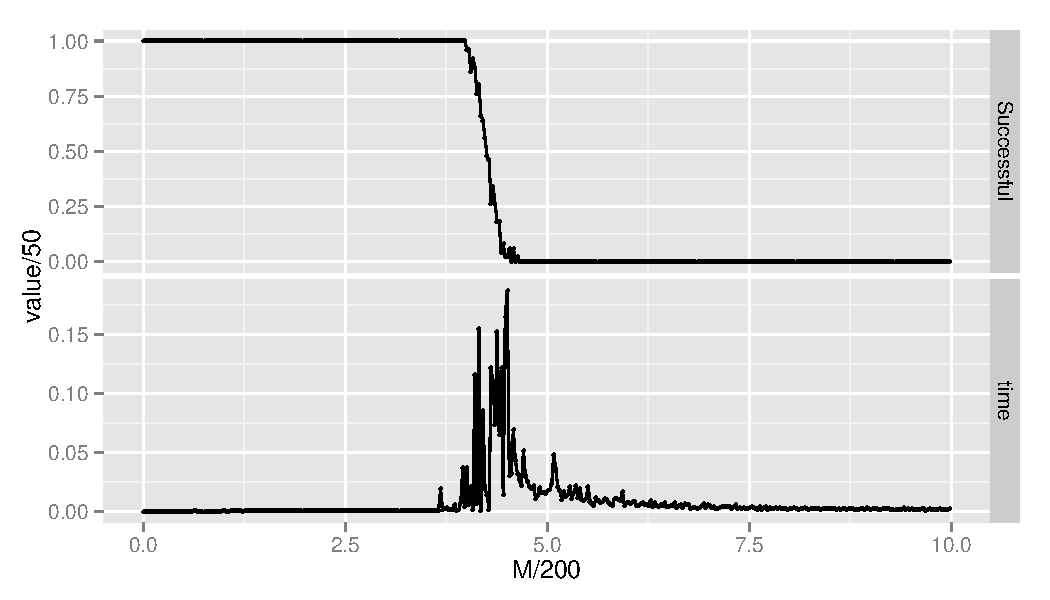
\includegraphics[width=.8\textwidth]{../material_2/plot_sat.pdf}
	\caption{Phase transition of SAT solving. In the lower figure the computational time for finding a solution for 3-SAT instances with a specific clauses-to-variables ratio (c/v-ratio) can be seen. The critical point is around $\alpha_{c} \approx $ 4.267 . In this regard, the upper figure shows the propability, whether these problem instances are solvable. So for the critical point it's hard to determine, whether a problem instance can be fulfilled with a concrete allocation or not. TODO Achsenbeschriftung value/50 M/200 erklären} \label{fig:crit_sat}
\end{figure}

In order to assess the solution quality of randomly generated 3-SAT instances we take the phase transition into account
and generate instances of every complexity region. More information about that in section Experimental Setup.

\subsection{Reduction from 3-SAT to Weighted Maximum Independent Set}
Since it can be shown that the Weighted Maximum Independent Set (WMIS) problem is equivalent to the Ising model \cite{choi2008minor}, the 3-SAT problem is first transformed into a WMIS problem, which can then be solved on an adiabatic quantum computer based on this equivalence.\\

The WMIS can be formulated as follows: Given is an undirected graph $\mathcal{G} = (V, E)$, where V is the set of vertices and E is the set of edges of $\mathcal{G}$, in which each vertice v $\in$ V is provided with a positive real weight $c_{v}$.\\
The problem is then to find a set S $\subset$ V, so that S is an independent set and the total weight of S, given by $\sum_{v \in S} c_{v}$, is a maximum. The optimal solution is also called WMIS($\mathcal{G}$).

The reduction from 3-SAT to WMIS is well known after \cite{choi2010adiabatic} and is for completeness recalled below.\\

\textbf{Reduction} (3-SAT $\leq_ {P}$ WMIS).
Given a 3-SAT instance $\Psi(x_{1}, \dots, x_{n}) = C_{1} \wedge ... \wedge C_{m}$ consisting of \emph{m} clauses \emph{($C_{1}, ..., C_{m}$)} and \emph{n = 3m} variables. Construct a graph $G_{SAT}$ as follows:
\begin{description}
	\item[Step 1:]\hfill \\
	For each clause $C_{i} = y_{i_{1}} \vee y_{i_{2}} \vee y_{i_{3}}$, $y_{j} \in \{x_{j}, \overline{x_{j}}\}$, a triangle is constructed, with the corners of the triangle being vertices labeled with the literals of this clause ($y_{i_{1}}, y_{i_{2}}, y_{i_{3}})$. Therefore the graph $G_{SAT}$ consists of 3m vertices.
	\item[Step 2:]\hfill \\
	Edges are added between vertices of different triangles if their labels conflict. That is, for two different triangles \emph{i} and \emph{j}, \emph{i} $\neq$ \emph{j}, which represent clause \emph{i} and \emph{j}, an edge is added, if there are variables $y_{i_{s}}$ and $y_{j_{t}}$, so that $y_{i_{s}} = \overline{y_{j_{t}}}$.
\end{description}

By doing this reduction the theorem after \cite{choi2010adiabatic} states, that an arbitrary 3-SAT formula $\Phi$, consisting of \emph{m} clauses, can be fulfilled, if the graph $G_{SAT}$, which was created by reducing $\Phi$ to a WMIS problem, has a WMIS of the size \emph{m}. 
This assertion represents an important relation between the satisfiability of a 3-SAT problem and the solution of the WMIS problem, which we take into account in this work.\\

For the sake of completeness we have to mention, that D-Wave's quantum annealer is designed to find the lowest energy state of a spin glass system, described by an Ising Hamiltonian (see equation \ref{eq:ising}). Here $ h_{i}$ is the on-site energy of qubit i, $J_{ij}$ are the interaction energies of two qubits i and j, and $s_{i}$ representing the spin (-1, +1) of the i-th qubit. So in order to execute the WMIS problem on the quantum annealing hardware , it has to be mapped to the Ising model. However, in \cite{choi2008minor} proof is given, that the WMIS problem is equivalent to the Ising model and no more modifications have to be made.

\begin{equation}\label{eq:ising}
	\mathcal{H}(s) = \sum_{i} h_{i}s_{i} + \sum_{i<j} J_{ij}s_{i}s_{j}
\end{equation}

